\documentclass[12pt, letterpaper]{article}
\usepackage{geometry}
 \geometry{
 a4paper,
 left=25mm,
 right=25mm,
 top=20mm,
 bottom=18mm
 }
\usepackage[utf8]{inputenc}
\usepackage{graphicx}
\graphicspath{ {images/} }
 
\title{COVID-19 data visualisation using coco}
\author{Rubaba Mammadova}
\date{\today}

\begin{document}
\maketitle

\begin{abstract}
This project focuses on the determination of countries that suffered most from the spread of COVID-19. 
\end{abstract}

\section{Dataset}

In my project, I used the data available from the site of World Health Organization (https://covid19.who.int/table) that contains information about cases and deaths in various countries.

\section{Third-party package coco}

I used third-party Python package called country\_converter which is a library to convert and match country names between different classifications and between different naming versions ("https://github.com/konstantinstadler/country\_converter").

Using classification scheme ISO3 that coco provides, I visualised country names that have higher number of total cases, total deaths and death rates in ISO3 format.
\section{Impact of COVID-19 }

While exploring the data some interesting details were observed. As you can see in the figure \ref{fig:plot1}, the top 10 countries with higher number of cases are USA, Brazil, India, Russian Federation, South Africa, Mexico, Peru, Chile, Columbia and Iran. However, top 10 countries with higher number of deaths are USA, Brazil, Mexico, The United Kingdom, India, Italy, France, Spain, Peru and Iran.

From here, it is visible that countries that have more cases are not always countries that the number of cumulative deaths are high. That is why, I decided to calculate the death rate in countries. In order to define the death rate in countries I divided the cumulative number of deaths to the total number of cases. As you can see in the figure \ref{fig:plot2}, the top 10 countries where death rate is too high are Yemen, France,The United Kingdom, Belgium, Italy, Hungary, British virgin Islands, Sint Maarten, Netherlands and Mexico. 

\section{Conclusion }

In conclusion, I can say that that Yemen, Belgium, Hungary, British virgin Islands, Sint Maarten and Netherlands were neither top10 countries with higher number of cases nor deaths but actually COVID-19 has impacted them more than other countries.  

 \begin{figure}[h]
    \centering
    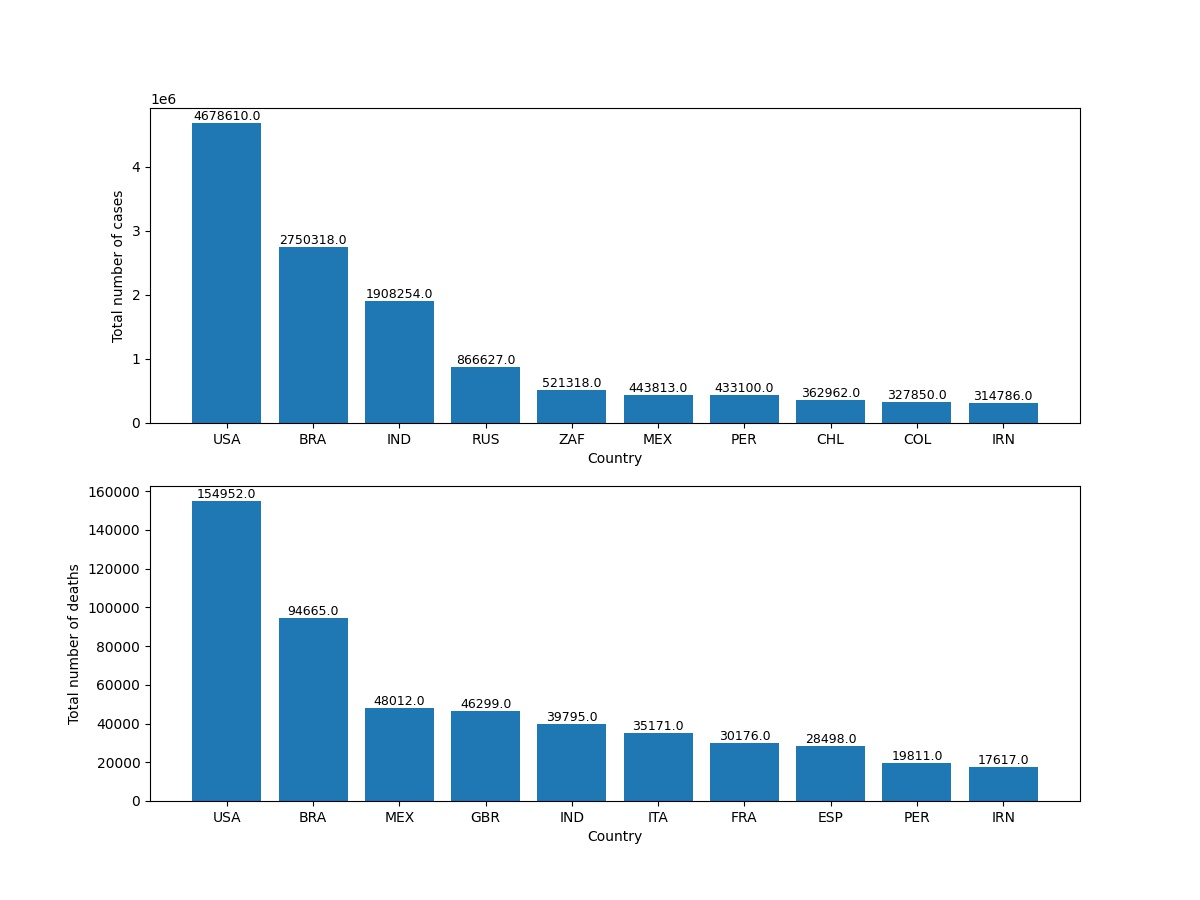
\includegraphics[width=1.1\textwidth]{plot1}
    \caption{Top 10 country cases and deaths}
    \label{fig:plot1}
\end{figure}


\begin{figure}[h]
    \centering
    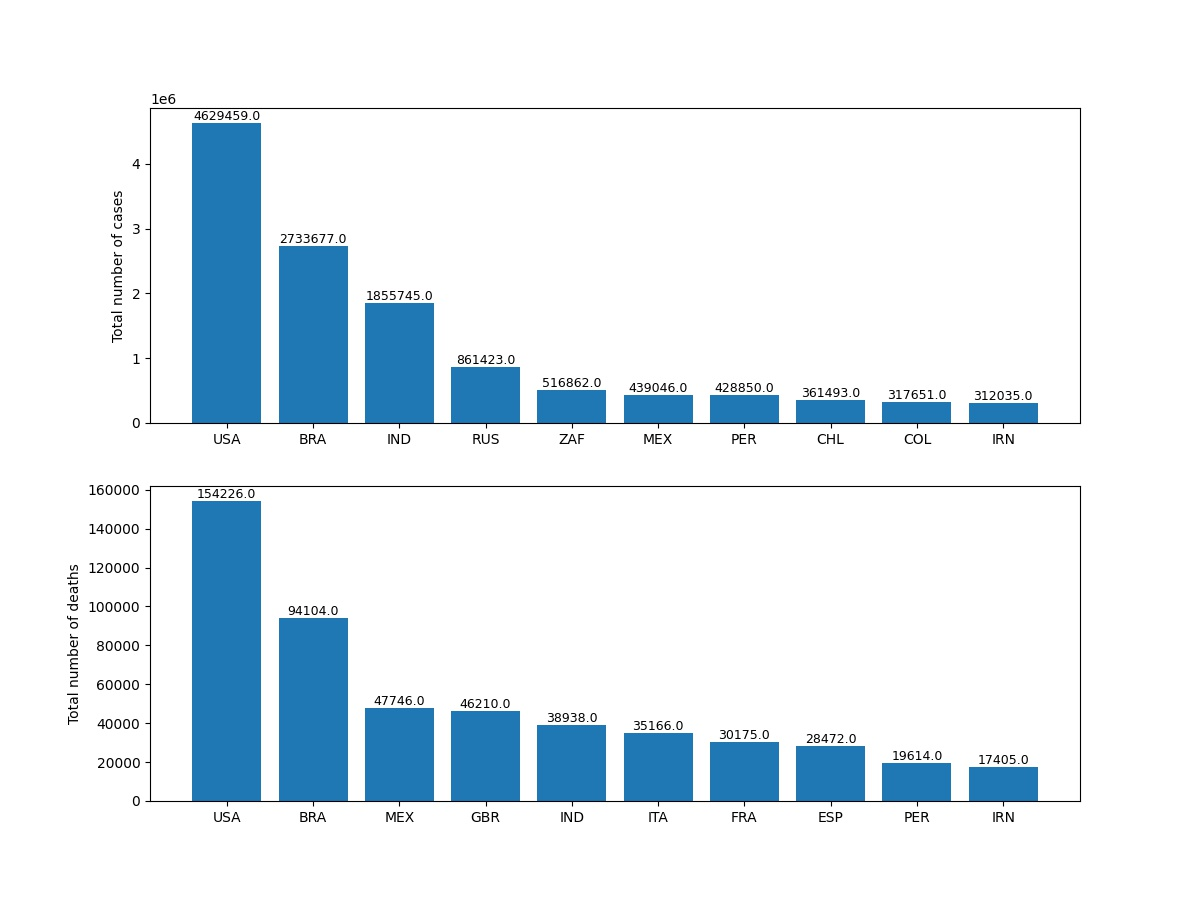
\includegraphics[width=1\textwidth]{plot2}
    \caption{Top 10 death rates}
    \label{fig:plot2}
\end{figure}

\end{document}